\documentclass[titlepage]{article}
\usepackage[utf8]{inputenc}
\usepackage{graphicx,wrapfig}
\graphicspath{{images/}}
\usepackage{amsmath}
\usepackage{wrapfig}
\usepackage{subcaption}
\usepackage{array}
\usepackage{float}
\usepackage[export]{adjustbox}
% ADDITION
\setlength{\parindent}{0pt}
% --------
\usepackage{geometry}
 \geometry{
 a4paper,
 total={170mm,257mm},
 left=20mm,
 top=20mm,
 }
\usepackage[utf8]{inputenc}
\usepackage[english]{babel}
\usepackage{fancyhdr}
 
\pagestyle{fancy}
\fancyhf{}
\fancyhead[LE,RO]{Nihaar Shah}
\fancyhead[RE,LO]{lady4932}
%\fancyfoot[CE,CO]{\leftmark}
\fancyfoot[LE,RO]{\thepage}
 
\renewcommand{\headrulewidth}{2pt}
\renewcommand{\footrulewidth}{1pt}
\usepackage{listings}
\usepackage{color}

\definecolor{dkgreen}{rgb}{0,0.6,0}
\definecolor{gray}{rgb}{0.5,0.5,0.5}
\definecolor{mauve}{rgb}{0.58,0,0.82}

\lstset{frame=tb,
  language=Matlab,
  aboveskip=3mm,
  belowskip=3mm,
  showstringspaces=false,
  columns=flexible,
  basicstyle={\small\ttfamily},
  numbers=none,
  numberstyle=\tiny\color{gray},
  keywordstyle=\color{blue},
  commentstyle=\color{dkgreen},
  stringstyle=\color{mauve},
  breaklines=true,
  breakatwhitespace=true,
  tabsize=3
}

\title{B1 report-Calibrating a camera}
\author{Nihaar R Shah}
\date{18 January 2016}

\begin{document}

\maketitle
%Introduction to the document
\section{Introduction}
Resectioning or calibrating a camera means to estimate the parameters of the lens and the sensor device of the camera. In order to estimate these parameters you need to have 3D world coordinates and their \textit{corresponding} 2D image points using multiple images of some calibration pattern. Assuming there aren't any inaccuracies (due to noise or outliers) in these correspondences and the position of camera relative to object is known then we can simply apply equations to obtain the required parameters. \\
However, in reality there will always be errors in matching up the corresponding points of image distance between a projected point and a measured one. We can apply RanSac algorithm to reduce outliers by choosing the best fitting points only. Secondly assuming the noise in the correspondences is mainly Gaussian noise, we can minimize the variance between these image locations and predicted locations. This optimization is known as bundle–adjustment. Our project implements these two procedures to find a close to accurate K-Matrix of required parameters.
% Aim and motivation subsections of Intro
\subsection{Aim}
The aim is to estimate and optimize the intrinsic parameters of a simplified ideal pinhole based model of a camera. My report attempts to \textit{test} and \textit{explain} the algorithms used and suggests further actions that can be taken to achieve a commercial solution.
\subsection{Motivation}
Knowledge of intrinsic parameters is very useful in finding real world distances of planar objects (from a single camera) if we know the position where the camera is mounted. Inversely, if we know distances in an image then we can estimate the camera location.\\
Using stereo cameras we can estimate depth as well, which is useful in \textbf{visual odometry} which has many applications in robotics for example in localization for \textbf{self-driving cars}.
% Specifications of the camera K matrix subsection of Intro
\subsection{Camera Model Specifications}
We have used an ideal pinhole simplification \textit{excluding} effects of radial and tangential lens distortion. The 5 intrinsic parameters are chip width and height, focal length (f), effective width and height of pixel, skewness $(\alpha)$ and principal point effects in x and y directions ($t_u$, $t_v$).The K-Matrix describes how the image in the unit camera is transformed into the real camera as an affine transformation.
%
% The KMatrix equation 
\begin{equation} \label{KMatrix}
K=
  \begin{bmatrix}
  \alpha f & \gamma f & t_u \\ 
  0        & \beta f  & t_v \\ 
  0        &    0     &  1 
  \end{bmatrix}
\end{equation}
%Starting a new section
\section{Outline}
The three main tasks in this project and their corresponding equations are as follows:
% Simulation subsection of Outline
\subsection{Simulation}
In practice we would use an actual calibration object like a checkerboard pattern with known distances between the edges.
In this project we are simulating the calibration object instead of using an image of a real world object to build our point correspondences between object and image. We use a known K-matrix using pre-defined parameters to make these correspondences unlike in practice.\\ 
In reality the K matrix is unknown. Through some other computer vision algorithm edge detection of the calibration object edges is possible. We manually then feed the known distances between these edges of the calibration object into the program to build the correspondences. In addition we input the 6 degrees of freedom needed to define the location of object in world coordinates. Instead, in this project we have functions to position the camera and position the object in world coordinates. A good test that these functions are working as expected is to view a simulated cube as seen by the camera as shown in figure (1). Note the 4 MegaPixel(MP) camera hence 2000 x 2000 pixel dimensions of the image.\\
\begin{figure}
\begin{subfigure}{0.5\textwidth}
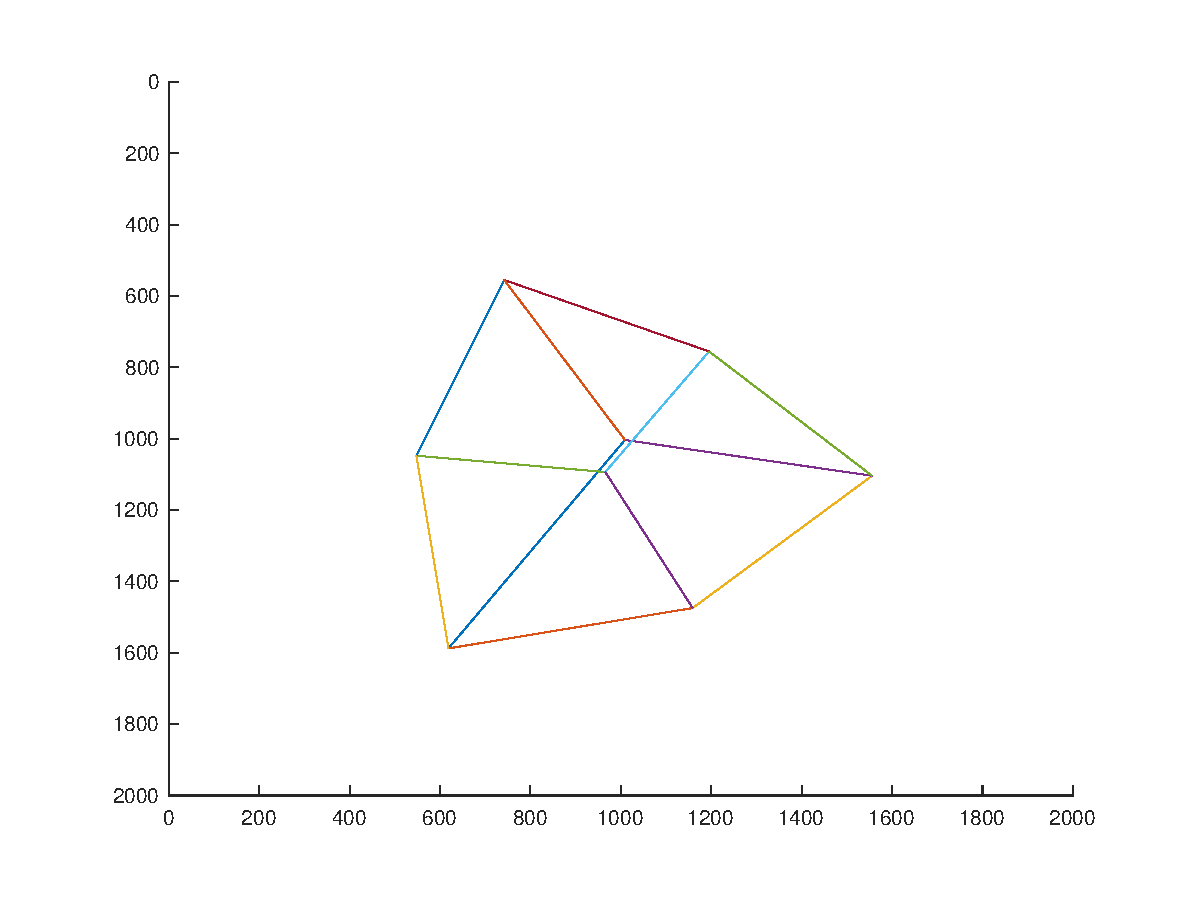
\includegraphics[width = 3.5cm,height = 3.5cm]{SimulateCube.eps}
\caption{Simulated cube in camera's field of vision.}
\label{wrap-fig:9}
\end{subfigure}
% Build noisy image figure
\begin{subfigure}{0.5\textwidth}
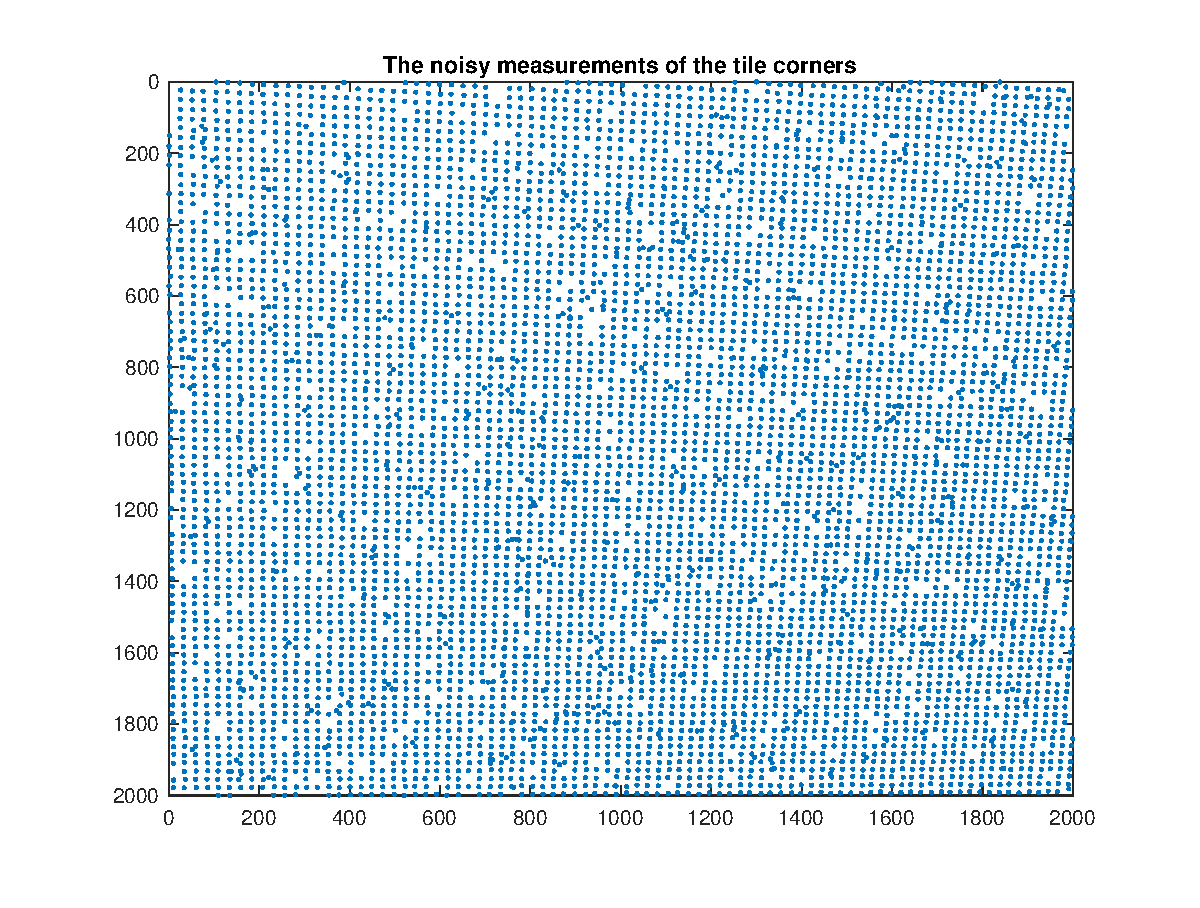
\includegraphics[width = 4.5cm,height = 4.5cm]{GridImage.eps}
\caption{Noisy grid image appears on camera sensor.}
\label{noisy-grid}
\end{subfigure}
\end{figure}
%
% Subsection on Estimation
\subsection{Initial Estimate}
\subsubsection{Estimating Homography}
% The object to image conversion equation 
\begin{equation}\label{uv-to-xy}
\begin{bmatrix}
  U\\ 
  V\\ 
  S 
  \end{bmatrix}
        = \textbf{K}
         \begin{bmatrix}
 \textbf{r1} & \textbf{r2} & \textbf{t}
         \end{bmatrix}
        \begin{bmatrix}
  x\\ 
  y\\ 
  1 
  \end{bmatrix}    
       =  \begin{bmatrix}
  h_{11}  & h_{12} & h_{13} \\ 
  h_{21}  & h_{22} & h_{23} \\ 
  h_{3_1}  & h_{32} & h_{33} 
  \end{bmatrix}
          \begin{bmatrix}
  x\\ 
  y\\ 
  1 
  \end{bmatrix}    
        \end{equation}
Equation 2 shows how we build point correspondences between object coordinates (xy) and image points (uv) from our checkerboard. Note how our required \textbf{K} parameters and the positional parameters are packed in the Homography elements $h_{i,j}$ and our task now becomes to estimate \textbf{H}. Equation 3 can be obtained by rearranging Equation 2.
%
% The object to image conversion equation 
\begin{equation}
    \label{Regressor}
  \begin{bmatrix}
  u\\ 
  v
  \end{bmatrix}
        = 
       \begin{bmatrix}
 x & y & 1 & 0 & 0 & 0 & -ux & -uy \\
 0 & 0 & 0 & x & y & 1 & -vx & -vy
  \end{bmatrix}
  \begin{bmatrix}
  h_{11}\\ 
    .\\
    .\\
  h_{32}
  \end{bmatrix}
 \implies \mathbf{p}_{j} = \mathbf{\phi}_{j}  \mathbf{h}_{j}
      \end{equation}
Using j = 1 to 4 known point correspondences we can stack the 4 matrices to build a determinate system of equations having 8 unknowns and 8 equations. Solving this system will give us an estimate of Homography. But how do we know that the 4 points we have chosen to estimate it are all inliers? Thus we perform RanSac to select those piexel points which fit well with the \textbf{H}. Now we have an over-constrained system with as many equations as the inliers. This system of equations is shown as in Equation \ref{System of Equations}. 
%
% The least squares minimum
\begin{equation}
    \label{System of Equations}
    \mathbf{P} =  \mathbf{\Phi} \mathbf{H}
    \end{equation}
We expect the correspondences to be noisy, hence no exact solution will exist. We therefore use \textbf{least squares minimization} as shown in Equation (5).
\begin{equation}
\label{Least Squares}
min |\mathbf{\Phi} \mathbf{H} - \mathbf{P}|^2 \implies \frac{\partial {|\mathbf{\Phi} \mathbf{H} - \mathbf{P}|^2}}{\partial\mathbf{(parameters)}} = 0 \implies \mathbf{H} = [\mathbf{\Phi}^T \mathbf{\Phi}]^{-1} \mathbf{\Phi} \mathbf{P}
\end{equation}
$\Phi$ (i.e. Regressor made of uv and xy coordinates) and \textbf{P} (i.e. uv coordinates) are \textit{known}. We use \textbf{singular value decomposition} (svd) to compute the inverse in Equation 5 because that is computationally cheaper than using matlab inverse. This is called pseudo-inverse. (See discussion in approx. and assumption section 3). Now we have computed an estimate of the Homography.
\subsubsection{Estimating K-Matrix from Homography}
\label{estK}
Finally we want to estimate the K matrix from this Homography using 3 images of the grid taken from different angles. Equation \ref{K from H} shows how we pre-multiply both sides by K inverse.
% K from H equation
\begin{equation}
    \label{K from H}
    \mathbf{H_j} = \lambda_j \mathbf{K_j} [\mathbf{r_1} \mathbf{r_2} \mathbf{t}]_j \implies \mathbf{K}^{-1} \mathbf{H_j} = \lambda_j [\mathbf{r_1} \mathbf{r_2} \mathbf{t}]_j
    \end{equation}
We use the orthogonal property of the rotation matrix by pre-multiplying the Homography with the rotation matrix transpose (or inverse) to get Equation \ref{inverse-transpose}.
    \begin{equation}
    \label{inverse-transpose}
        \mathbf{H_j}^T (\mathbf{K^{-1}})^{T} \mathbf{K_j}^{-1} \mathbf{H_j} = \lambda^2 \mathbf{I}
    \end{equation}
This equation holds true for each image j and can be used to make a homogeneous equation of form Ax=0 to solve for ${\mathbf{phi}} = (\mathbf{K}^{-1})^T \mathbf{K}^{-1}$ again using svd(\textbf{A}) = \textbf{U} \textbf{D} \mathbf{$V^T$} and right singular vector of matrix \mathbf{$\phi$} associated with the \textit{smallest} singular value. This is because for a homogeneous system any vector \mathbf{x} in the null space of \textbf{A} is a solution hence any column of \mathbf{V} whose corresponding singular value is zero is a solution. If we want a particular solution then we might want to pick the solution \mathbf{x} with the smallest length $|\mathbf{x}|^2$. We then obtain \textbf{K} from $\Phi$ using \textit{cholesky factorization} because we note that $(\mathbf{K}^{-1})^T$ is an upper triangular matrix and $K^{-1}$ a lower triangular matrix.{see discussion later?}
% Starting subsection called Optimization
\subsection{Optimization}
So far we have gotten rid of outlier effects to an extent using RanSac. However Gaussian noise (in this project which was artificially added) still prevails. We can tackle this Gaussian noise using optimization of the cost-function (\textbf{E}) defined as the least squares error between estimated and true values of uv.
\begin{equation}
E =\frac{1}{2} \Sigma(Estimated [u'v'] - True [u v])^2
\end{equation}
 Note that least squares form of cost function is an efficient way to eliminate noise but not outliers as it heavily penalizes Outliers. Thus, we have chosen the two step approach - RanSac followed by least squares optimization. \\
This is a convex optimization problem (since the cost function is quadratic) hence we should expect the global minimum and local minimum to be the same. We decompose the Homography into the K-Matrix and positional parameters and then use this to predict the positions of points in the image using these transformation matrices and the current best camera matrix. The square of this minus the actual positions serves as our convex cost function.\\
We will use the \textbf{Levenberg-Marquardt algorithm} to adjust parameters and decide when the minimum is reached. Steepest descent is a method to reach minimum by varying parameters $\delta$ \textbf{p} along the steepest \textit{downhill} direction on the surface i.e. pointing along the \textit{negative} gradient vector.
% Gradient descent equation
\begin{equation}
\label{steepest_descent}
\delta \textbf{p} = -(\frac{\partial \mathbf{E}}{\partial\mathbf{p}})^T = g_n
\end{equation}
%  
Newton steps method is based on taking the derivative of Taylor's expansion in N-dimensions as shown in Equation \ref{Newton_Step}   
% Newton step equation 
\begin{equation}
  \label{Newton_Step}
  \nabla (f(\textbf{x}+\delta\textbf{x}))=0 \implies \mathbf{g_n} + \mathbf{H_n} \delta p = 0\\
  \implies \delta{\mathbf{p}}=-\mathbf{H_n}^{-1}\mathbf{g_n}
\end{equation}
This gives the iterative update $\mathbf{x_{n+1}}=\mathbf{x_n}-\mathbf{H_n}^{-1} \mathbf{g}_n$ where $\mathbf{H_n}$ is the Hessian matrix $\frac{\partial^2 \mathbf{E}}{\partial \mathbf{p}^2}$. It is better to perform line search which ensures global convergence hence we introduce the parameter $\mu$ in Equation \ref{Newton_Gradient}
% Newtonstep-Gradient descent  equation 
\begin{equation}
\label{Newton_Gradient}
\mathbf{x_{n+1}}=\mathbf{x_n}-\mu\mathbf{H_n}^{-1} \mathbf{g}_n
\end{equation}
Combining Equations \ref{Newton_Step} and \ref{Newton_Gradient} we get:
\begin{equation}
  \label{Final_Newton_Gradient}
  (\mathbf{H_n}+\mu\mathbf{I})\delta \mathbf{p}= -\mathbf{g}_n
\end{equation}
By solving for $\delta$\mathbf{p} we we know the vector along which to change our parameters for the next iteration. We re-compute the cost at the new parameters and assess whether to reject the parameters or accept them as well as whether to increase or decrease $\mu$ i.e. we can control between Newton steps and gradient descent.
%-------------------------------------------------------------------------------------------------------
% Start section on the overview of structure
\section{Overview of the Structure}
\subsection{Data Structure}
\subsection{Control Path}
\textbf{RanSac flow}\\
RanSac is an algorithm to eliminate outlier points - in this case pixels that may be displaced from their true positions in the calibration image. While estimating homography from the edges of the checkerboard we take 4 random point correspondences to build our regressor $\Phi$ as seen in Equation 4. To ensure these points are a true representation of the objects (inliers) we perform RanSac.\\
%
We shall use RanSac so we can use \textit{that} homography estimate which best agrees or is most representative of maximum number of points on the checkerboard. The flowchart in Figure \ref{Ransac_Flow} shows this algorithm.\\
Note that UV cordintes are the known points or true points. We multiply the estimated homography with the xy object coordinates to obtain estimated U’V’. RanSac compares the difference between the U’V’ estimated via homography and the true UV with a threshold MaxError and populates a vector of points that satisfies this threshold as acceptable inliers. \\
This set is called Best Consensus and then we construct our Regressor of the over-constrained system (Equation\ref{System of Equations}) and use svd to find the least squares estimate of our final homography if the condition number is “good” i.e.
well conditioned system hence accurate inverse is possible. Once we have a good homography estimate it is straightforward to compute K using svd as mentioned in Section \ref{estK}.\\
\textbf{Optimization flow}\\
The algorithm controls the search to move from steepest descent to newton steps depending on how well the last search performed. \\
The feedback mechanism is that if the error has increased after changing the parameters along a certain direction (computed in Equation \ref{Final_Newton_Gradient}) then the weighting $\mu$ is increased reducing the step-size and causing the algorithm to just search downhill. If on the other hand the error has reduced that means we are \textit{closer} to the minimum so we search in the neighborhood itself using Newton steps.\\
\begin{center}
\textbf{FlowCharts for Algorithms used}\\
\end{center}
\begin{figure}[H]
\begin{subfigure}{0.5\textwidth}
   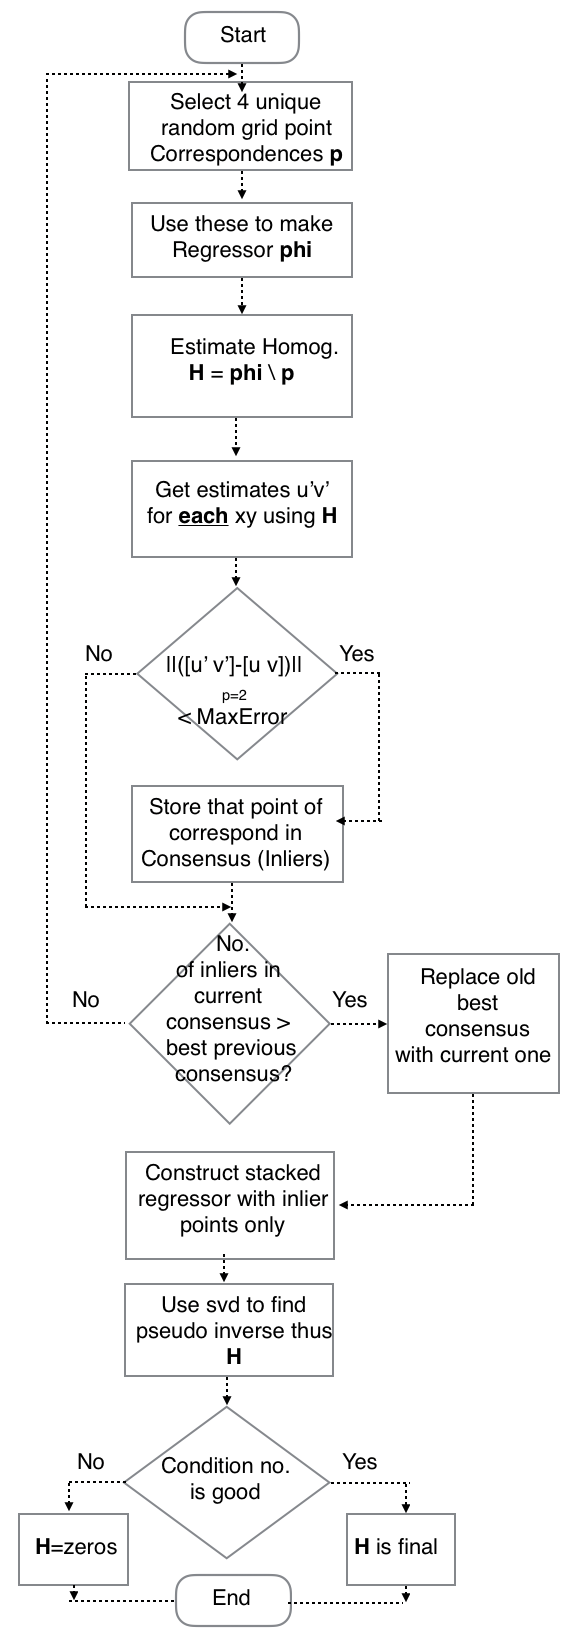
\includegraphics[width = 7cm,height = 18cm]{Ransac_flowchart.png}
   \caption{Estimation task involving RanSac}
   \label{Ransac_Flow}
\end{subfigure} 
\begin{subfigure}{0.5\textwidth}
    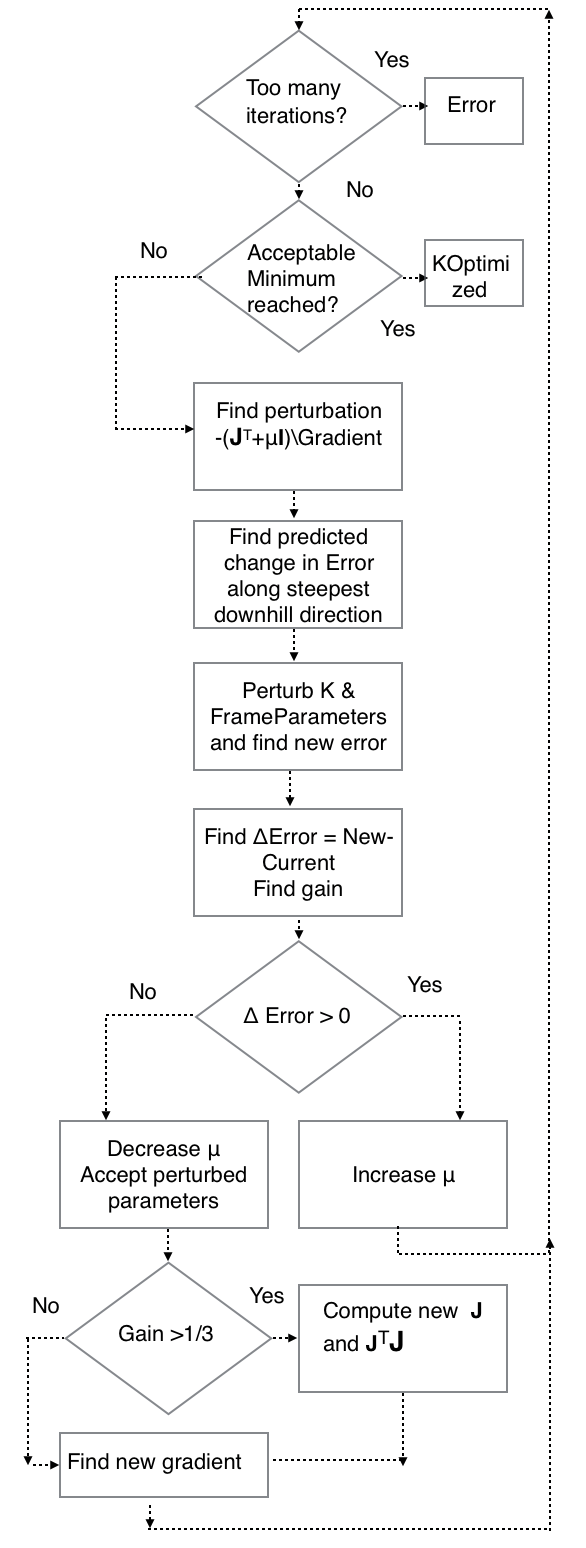
\includegraphics[width = 7cm,height = 18cm]{optim-flowchart.png}
    \caption{Optimization:the L-M algorithm}
  \label{Optim_Flow}
\end{subfigure} 
\caption{Flow charts for the two algorithms used to reduce Outliers and Noise respectively.}
\end{figure}
\subsection{Why our approach?}
\begin{figure}[H]
\begin{subfigure}{0.5\textwidth}
   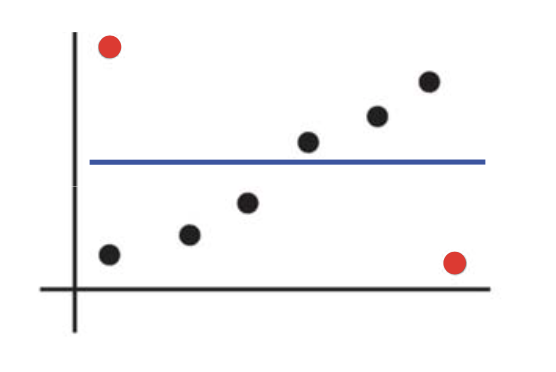
\includegraphics[width = 4cm,height = 4cm]{outlier.png}
   \caption{Outliers}
   \label{Ransac_Flow}
\end{subfigure} 
\begin{subfigure}{0.5\textwidth}
    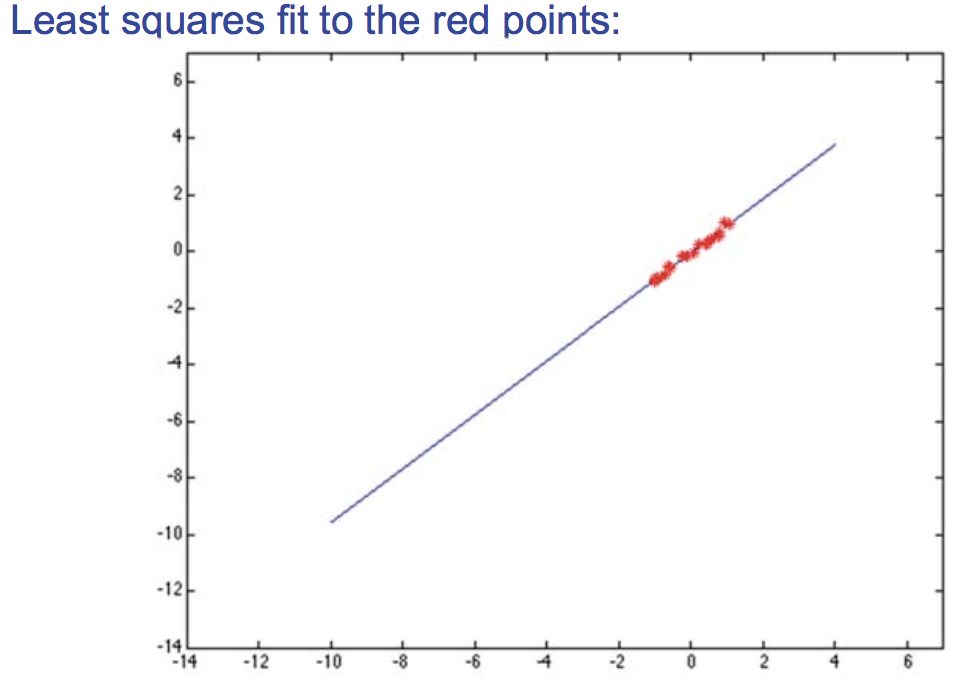
\includegraphics[width = 4cm,height = 4cm]{noise.png}
    \caption{Noise}
  \label{Optim_Flow}
\end{subfigure} 
\caption{Graphical representation of impact of Least Squares minimization on Noise and Outliers.}
\end{figure}
Suppose you fit a straight line to data containing outliers, the usual method of least squares estimation is flawed. It will penalize outliers excessively and lead to poor fit. Thus we must first get rid of these outlier and \textbf{then} apply Least Squares optimization. This is precisely our method.

%-------------------------------------------------------------------------------------------------------
\section{Detailed Considerations}
\subsection{How to measure accuracy}
\label{Accuracy}
%
% screenshot of correspond variable data structure
\begin{figure}[H]
\begin{center}
\begin{subfigure}{0.5\textwidth}
\label{Correspond}
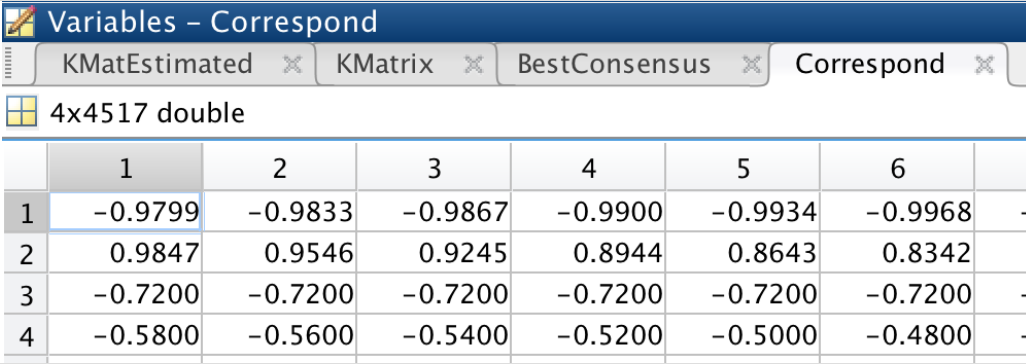
\includegraphics[width = 14cm,height = 2.5cm,center]{Correspond_workspace.png}
\caption{Values stored inside Correspond. Number of columns represents total points on the grid.}
\end{subfigure}\\
% screenshot of consensus data structure
\begin{subfigure}{0.5\textwidth}
\label{Consensus}
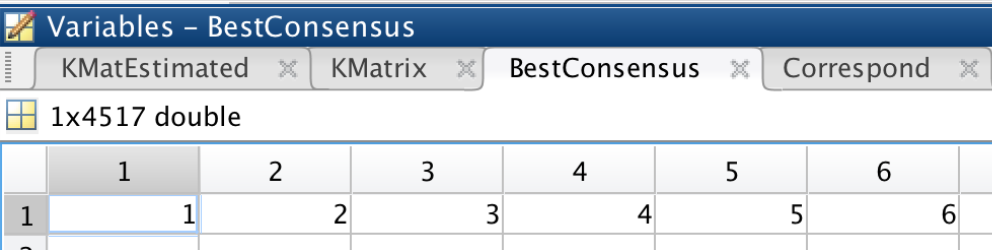
\includegraphics[width = 14cm,height = 2.5cm,center]{BestConsensus_workspace.png}
\caption{Dimensions verify BestConsensus vector contains all points on the object i.e. no outliers.}
\end{subfigure}
%\caption{Workspace data structures showing Correspondences and Consensus matrices}
\caption{The workspace data structure dimensions verify all points are inliers.}
\end{center}
\end{figure}
\textbf{\underline{Noise and Outlier Test}}\\
The simplest was to set the noise variance and mean to zero and set probability of outliers added also to zero in the Correspondences matrix.\\
\vspace{2mm}
\textbf{Hypothesis}: This would mean there are now \textit{only} inliers i.e. all point correspondences are accurate so estimating homography from any 4 points should give an error of approximately zero, since u’=u and v’=v. Thus \textit{no} points are excluded from Best Consensus vector. \\
\vspace{2mm}
\textbf{Result}: This was verified as seen in Figures 3 (a) and (b).\\
% 2nd experiment
\textbf{\underline{RanSac runs Test}}\\
The second experiment was to vary number of RanSac runs and examine its effects on the accuracy of $K_{estimated}$. The accuracy metric used was the $L_{1}$ norm because it is less susceptible to outliers than $p > 2$ norm and maybe more representative that p=0 or p=inf norm(?).\\
\textbf{Hypothesis}: More RanSac runs means more number of homographies to use for best fitting correspondence points hence a more accurate K estimate. The noise, variance and pOutlier were used as control parameters. \\
\textbf{Result}:The general trend corroborates this expectation as seen in Figure \ref{RansacRunsVsAccuracy}.
\begin{figure}[H]
\begin{center}
% Plot of ransac vs accuracy
\begin{subfigure}{0.25\textwidth}
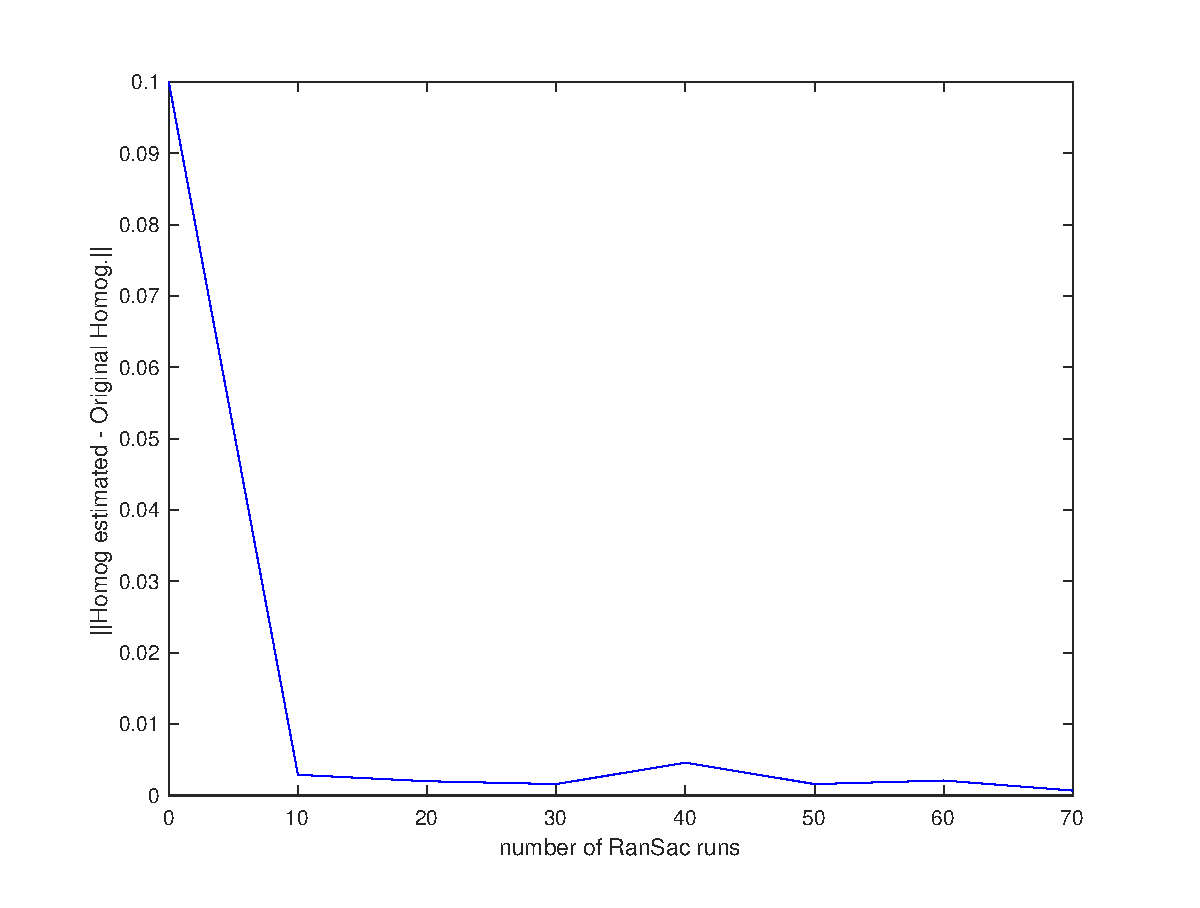
\includegraphics[width = 5cm, height=5cm,left]{HomogErrorVsRansacRuns.eps}
\caption{Number of RanSac runs.}
\label{RansacRunsVsAccuracy}
\end{subfigure}\hspace{2cm}
% Plot of MaxError vs accuracy
\begin{subfigure}{0.25\textwidth}
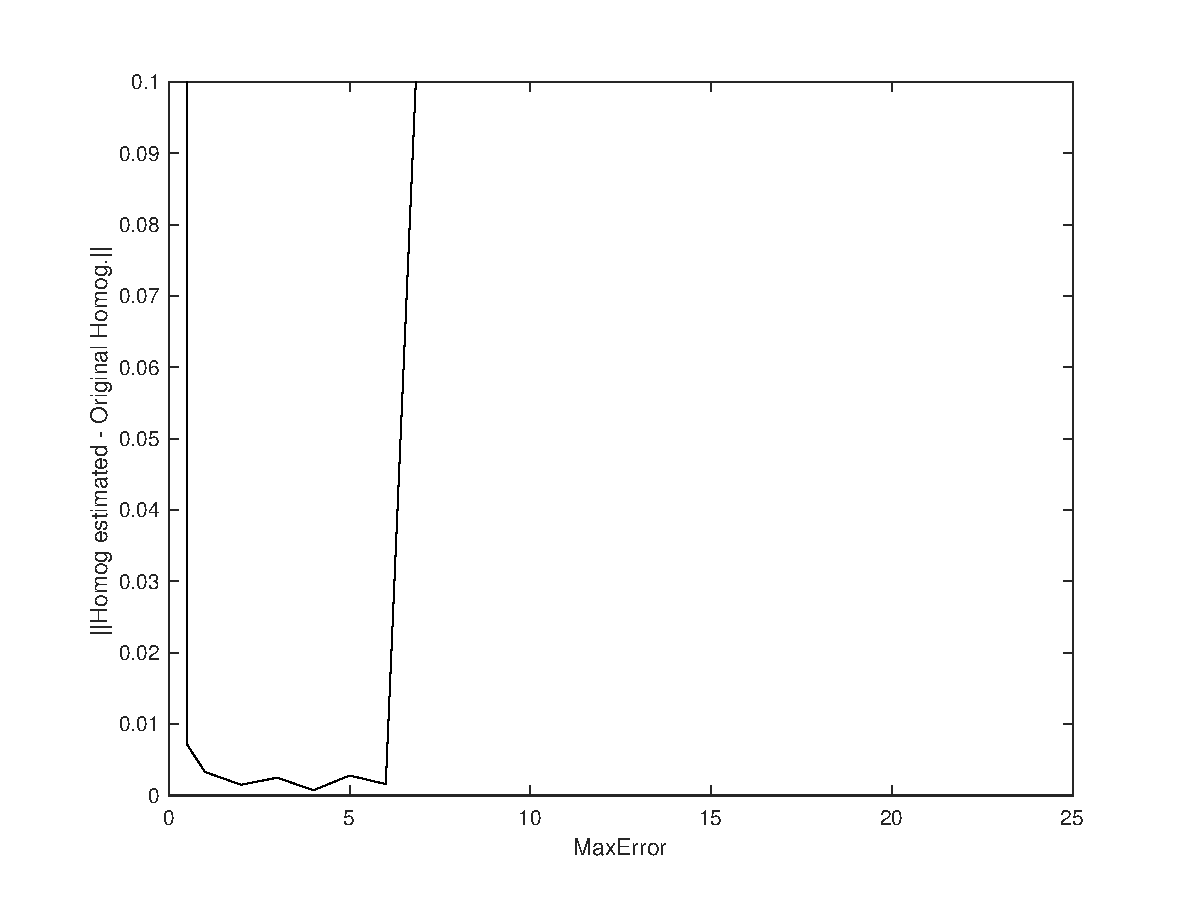
\includegraphics[width = 5cm, height=5cm,right]{MaxErrorVsHomogError.eps}
\caption{MaxError in RanSac.}
\label{MaxErrorVsAccuracy}
\end{subfigure} 
\caption{Varying Ransac runs and MaxError to find effect on Accuracy.}
\end{center}
\end{figure}
\textbf{\underline{MaxError Test}}\\
% 2nd experiment of Maxerror vs accuracy
\textbf{Hypothesis}: Similarly changing the MaxError value will have an effect on the accuracy of our estimate. Increasing the MaxError means we are increasing the threshold accuracy for an estimated u'v' to be part of consensus set. So we will have more strict inliers for higher MaxError hence more accuracy.\\

\textbf{Result}:The result was that both for very high or very low MaxError values the accuracy drops. This is because of \textbf{over-fitting}. If the max error is too low, there will be very few points in the consensus hence the regressor for the robust inverse calculation will have too few points. This is also risky for our estimate. I have made the script also output how many points are there in best consensus set for a given Max Error value and found that for an error of $10^-4$ and a noise variance of 0.1 we just have 10 elements and this reduces if error is further reduced or if noise variance is increased. Too few points in consensus means when we use svd to find robust inverse and hence our Homography there are very few points and therefore a risk of overfitting. This can be seen in the poor accuracy $\|K_{estimated} - K_{matrix}\|$ for low Max Error in Fig. 4b 
% \vspace{2mm}
%
Other tests include: for zero noise and pOutlier = 0, K-Matrix estimated is the same as the K-Matrix.
% ADDITION
\bigskip

% --------
% \vspace{2mm} 
\textbf{\underline{Test for Jacobian calculation}} \\
For optimization I calculate the jacobian matrix with respect to 11 parameters by writing my own \textit{forward-difference} function. The perturbation was set to 0.001 \% of the parameter and we used a for-loop to manually differentiate with respect to each parameter and construct our blocks as shown in the code below:
%
 % insert code
\begin{lstlisting}
 % We are estimating the derivative using f'(x)=[f(x+dx)-f(x)]/dx w.r.t each of 11 parameters
 perturbation = 1.001;
for a = 1 : length(Correspond)
    % Extract corresponding point from NCORRESPOND
    b = NCONSENSUS(a);  % b selects each point in Consensus one by one
    XY = NCORRESPOND(3:4, b);   % Vector of xy inlier grid points
    UV = NCORRESPOND(1:2, b);   % Vector of uv inlier grid points
    
    % Calculate perspectivies by finding rotational matrix from Angle-axis
    ROTANG = norm(NANGLE);  % The axis of rotation is a unit vector times the angle of rotation
    ROTAXIS = NANGLE/norm(NANGLE);  % Divide by the norm to separately obtain the rot. angle and vector
    R = RodriguesRotation(ROTAXIS, ROTANG); % Constructs the rotation matrix from angle & vector
    P = [R(1:3,1:2) NTRANSLATION]; % Perspectivity is constructed from the rotation matrix and trans.
    
    % This is f(x)
    UVest = KMatrix * P * [XY;1]; % U'V' are estimated by multiplying Homography with XY
    UVest = UVest(1:2)/UVest(3);
    
    % Perturb each K parameter by a small percent of itself turn by turn and store each perturbed matrix
    k1 = KMatrix;
    k1(1,1) = KMatrix(1,1)*perturbation; 
    k2 = KMatrix;
    k2(1,2) = KMatrix(1,2)*perturbation;
    % ... and so on until k5(2,3)=KMatrix(2,3)*perturbation;
    
    % Find new estimated uv from each perturbed kmatrix. This is f(x+dx) in f'(x)=[f(x+dx)-f(x)]/dx
    fk1 = k1 * P *[XY; 1];
    fk2 = k2 * P *[XY; 1];
    % ... and so on until fk5 = k5 * P *[XY; 1];
    
    % This is f'(x). We divide by fk(3) to scale it back to original.
    dk1 = (fk1(1:2)/fk1(3)-UVest)/(KMatrix(1,1)*(perturbation-1));
    dk2 = (fk2(1:2)/fk2(3)-UVest)/(KMatrix(1,2)*(perturbation-1));
    % ... and so on until dk5;
    
    % Finally constructing our K parameters block consisting of 5 columns and 2*no. of points rows 
    NKMATJACOB(2*a-1:2*a,:) = [ dk1 dk2 dk3 dk4 dk5 ];
  end
\end{lstlisting}
%
 To \textbf{test the accuracy} of this function, I wrote another function using symbolic MATLAB toolbox which textbf{analytically} finds the \textit{entire} Jacobian and then I select the required blocks from that, as shown in the code below:
% insert more code
\begin{lstlisting}
function [J4,J8] = JacobianSym(KMatrixValues,RotValues,TranslationValues,CorrValues,BestConsensus)
% This function computes the entire jacobian matrix of 11 columns (for 11 parameters) and 2*nConsensus rows using symbolic toolbox. Then substitute the values and obtain the numerical jacobian automatically.
n = length(BestConsensus);
% Parameters come from KMatrix, Rotation axis and Translation vector
K = sym('k',[3,3]);
RotAxis = sym('rot',[1,3]);
t = sym('t',[3,1]);
Theta = norm(RotAxis);
Correspond=sym('cor',[4,n]);
fin = sym('fin',[2*n,1]);

% L is a matrix of rotaxis parameters. It is used to find the rotation matrix using Rodrigues formula.
L = [0, -RotAxis(1,3)/Theta, RotAxis(1,2)/Theta;RotAxis(1,3)/Theta,0,-RotAxis(1,1)/Theta;-RotAxis(1,2)/Theta,RotAxis(1,1)/Theta,0];
I = eye(3); % identity matrix 3x3

% Assembling the rotation matrix from the 3 rotation axis parameters packed in the L matrix
R = I + sin(Theta)*L + (1-cos(Theta))*L^2;

% Forming the Perspectivity from the Rotation axis parameters packed inside r1 and r2 and the Tanslation vector. Thus P contains all 6 extrinsic parameters- Rotation and translation
r1 = R(1:3,1);
r2 = R(1:3,2);
P = [r1,r2,t];
fin =[]; % initializing the matrix
% fin is calculated symbolically in terms of the 6 extrinsic parameters in P and 5 intrinisic in K
for i = 1:n
    XY = Correspond(3:4,BestConsensus(i));
    f = K * P * [XY' 1]';
    f = f/f(3);
    fin = [fin;f(1:2,1)];
end
Variables = [(1,1),K(1,2),K(1,3),K(2,2),K(2,3),RotAxis(1,1),RotAxis(1,2),RotAxis(1,3),t(1,1),t(2,1),t(3,1)];
% symbolically forming the two blocks using the jacobian library function
JKMat = jacobian(fin,Variables(1,1:5));
JFram = jacobian(fin,Variables(1,6:11));

% Substituting in the K parameter values
J1 = subs(JKMat,K,KMatrixValues);
J2 = subs(J1,RotAxis,RotValues');
J3 = subs(J2,t,TranslationValues);
J4 = subs(J3,Correspond,CorrValues); % Finally has all the required values subbed in. It is returned.

J5 = subs(JFram,K,KMatrixValues);
J6 = subs(J5,RotAxis,RotValues');
J7 = subs(J6,t,TranslationValues);
J8 = subs(J7,Correspond,CorrValues);% Finally has all the required values subbed in. It is returned.
\end{lstlisting}
%
MATLAB's 'jacobian' library function uses \textbf{central difference}. This is a more analytic kind of approach and is a more accurate measure than simply forward difference. However, this is extremely computationally expensive because even the zero-terms of the Jacobian are computed which can otherwise be avoided by only calculating the required blocks as done in the first of the two functions above.\\
Both results were nonetheless similar, thus we prefer the first method.
%
\subsection{Is this simulation a good model of the real world?}
\label{realistic}
There are approximations and assumptions in any model. Here are a few:
\textbf{I.I.D. Noise}
Principal sources of Gaussian noise in digital images arise during acquisition e.g. sensor noise caused by poor illumination and/or high temperature, and/or transmission e.g. electronic circuit noise. A typical model of image noise is Gaussian, additive, independent at each pixel. Obviously, there are other noise sources that are \textbf{Gaussian} e.g. Salt-and-pepper noise (caused by analog-to-digital converter errors), Shot noise (typically caused by statistical quantum fluctuations), Quantization noise (caused by quantizing the pixels of a sensed image to a number of discrete levels), Anisotropic noise (noise sources show up with a significant orientation) etc. Thus Gaussian noise is an \textbf{approximation} not totally representative of truth. Based on this assumption we even choose our cost function in optimization as a least squares minimization.
% ADDITION
\medskip

% --------
\textbf{Outliers}\\
An outlier in an (photographic) image pair is often a region that has been occluded, an object that suddenly appears in one of the images, or a region that undergoes an unexpected motion (due to slight camera motion). Outlier modelling is a field on its own. We have used a \textbf{simplistic} way of adding outliers at random pixels.
% ADDITION
\medskip

% --------
\textbf{Lens distortion}\\
Radial Distrortion occurs when light rays bend more near the edges of a lens than they do at its optical center. The smaller the lens, the greater the distortion.\\
Tangential distortion occurs when the lens and the image plane are not parallel. The tangential distortion coefficients model this type of distortion.\\
We have \textbf{assumed} an ideal pin-hole camera with no such distortions.
% ADDITION
\medskip

% --------
\textbf{Algebraic approximations}: \\
For mathematical and computational simplicity we have used certain approximations. For instance to caluclate matrix inverse we use svd \textit{'pseudo inverse'}. For determining stopping criterion, instead of comparing Gradient to 0 we set the criterion to a \textit{really low number} such as 1e-5. For computing the \textit{Hessian} as second partial derivatives we approximate it as $J^{T}J$ thus using the jacobian already calculated.
\section{Measures of Code Performance}
\subsection{Noise}
\begin{wrapfigure}{r}{5.5cm}
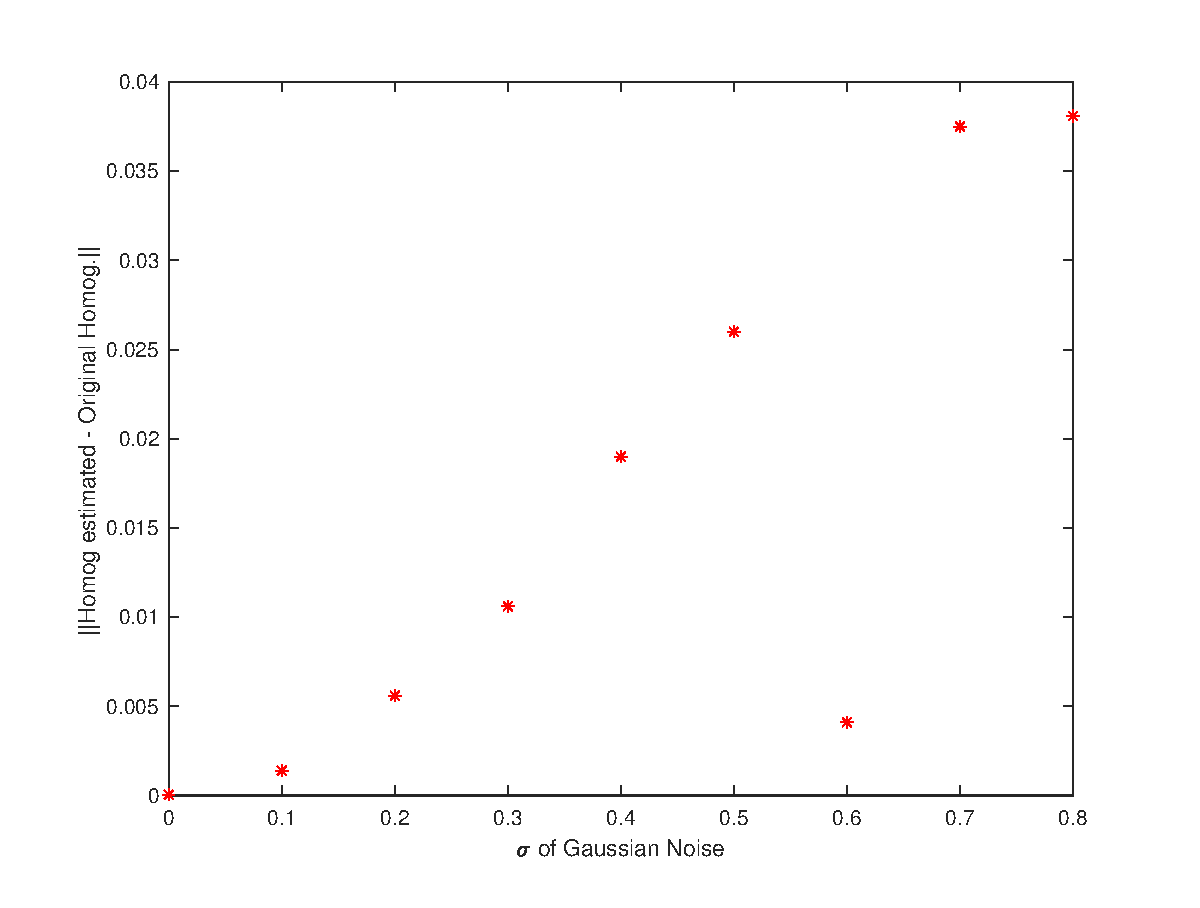
\includegraphics[width = 5.5cm, height=5.5cm]{HomogerrorVsNoiseVariance.eps}
\caption{Effect of varying noise variance on accuracy of estimation.}
\label{wrap-fig:1}
\end{wrapfigure} 
Trend is that more the noise variance i.e. the image pixels of calibration image are more apart from their true values then the worse the error between the Frobenius norm between true Homography matrix and the estimated. Although there is one outlier in the above trend, that is reasonable since we are randomly choosing points each time we run the estimate. So even with the same value of standard deviation and every other parameter, there will be variations in the error values which is why we can explain that as long as the trend is towards worse error with increased variance we can ignore this particular outlier in the above graph.
\subsection{Speed}
The Figure shows how the analytic jacobian compares with the forward difference method. The self-time (i.e. the time taken in that particular function excluding the 'child' functions) for finding the Jacobian compares so:
\begin{verbatim}
% improvement = 0.068/(0.264-0.068) = 35 %
\end{verbatim}
While the total time taken i.e. includes the cumulative time over all the iterations and Ransac runs is incomparable 0.497s vs 108.64s. Thus, we clearly prefer the approximate forward difference method.
% screenshot of correspond variable data structure
\begin{figure}[H]
\begin{subfigure}{0.5\textwidth}
\label{Correspond}
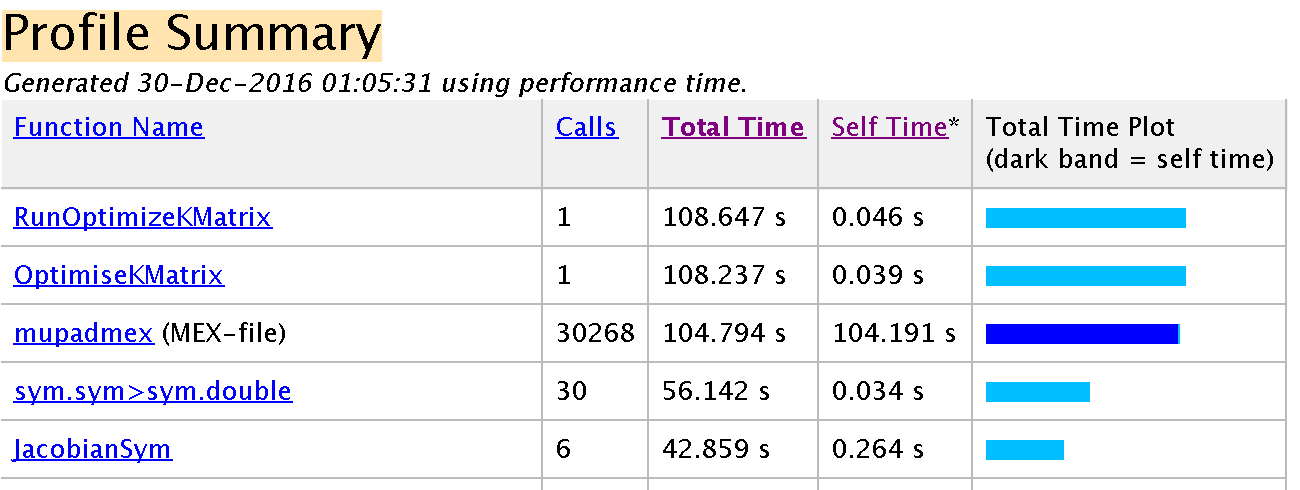
\includegraphics[width = 8.0cm,height = 3.5cm]{JacobianSym_timing.png}
\caption{Using library jacobian function.}
\end{subfigure}
% screenshot of consensus data structure
\begin{subfigure}{0.5\textwidth}
\label{Consensus}
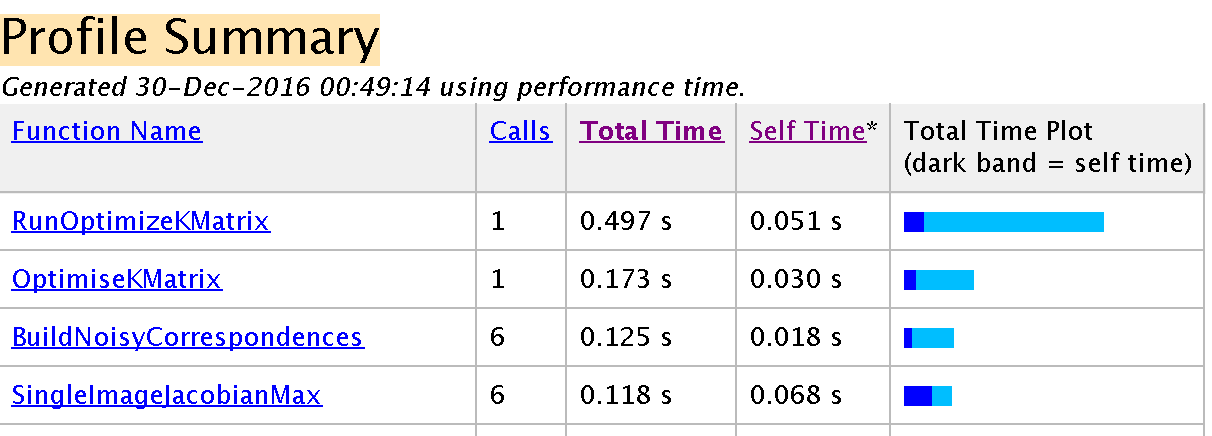
\includegraphics[width = 8.0cm,height = 3.5cm]{singleImageJacob_timing.png}
\caption{Using forward difference.}
\end{subfigure}
%\caption{Workspace data structures showing Correspondences and Consensus matrices}
\caption{Timing performance for the two methods to compute Jacobian.}
\end{figure}
\section{Conclusions}
\subsection{Assessment of Data Structures}
\subsection{How would I input real data?}
This project simulated the calibration image. In reality we would use an image of an actual calibration image and of-course after calibration we only deal with real world images. Edge detection is an important part of Image Processing where we can find boundaries of objects within image \textbf{by detecting discontinuities} in brightness. Common algorithms include Sobel, Canny, Prewitt, Roberts, and fuzzy logic methods. The MATLAB command:
\begin{verbatim}
BW = edge(I,<type of algorithm>,threshold,direction)
\end{verbatim}
returns a binary image BW containing 1s where the function finds edges in the input image I and 0s elsewhere. It returns edges that are stronger than threshold. The input image I is an intensity or a binary image. Once edges are detected then we can enter the known distances between them in the calibration image. After it is calibrated, we can use K-Matrix and Extrinisic parameters (from the position where we mount camera with respect to object) to find the real-world distances simply from an image of the planar objects. 
\subsection{How well did you do?}
\begin{figure}[H]
\begin{subfigure}{0.4\textwidth}
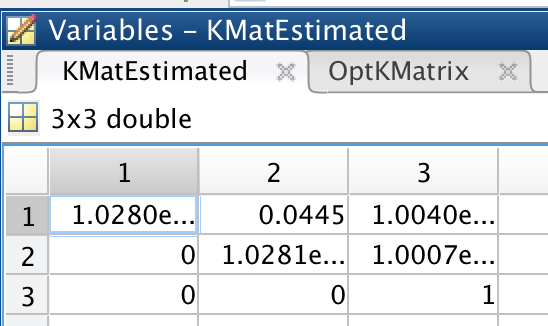
\includegraphics[width = 3.8cm,height = 2.5cm,center]{kestim.png}
\caption{Initial Estimated (NB: exponents are power 3.)}
\end{subfigure}
\begin{subfigure}{0.4\textwidth}
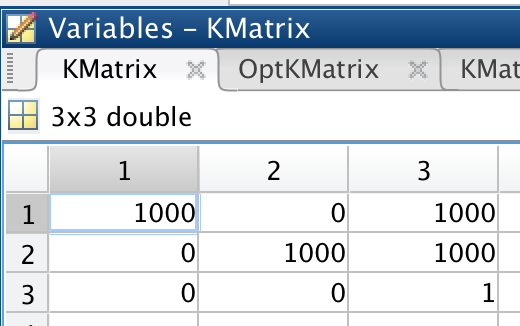
\includegraphics[width = 3.8cm,height = 2.5cm,left]{KAct.png}
\caption{Actual or true KMatrix.}
\end{subfigure}
% screenshot of consensus data structure
\begin{subfigure}{0.4\textwidth}
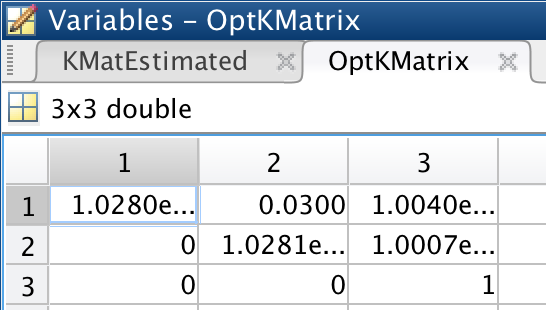
\includegraphics[width = 3.8cm,height = 2.5cm,right]{opt-kmat.png}
\caption{Optimized K-Matrix (nearly same as estimated)}
\end{subfigure}
\caption{Comparing the final K-optimized and K-Estimated. Noise $\sigma$ =0.2, Stopping criterion value =1e-8 }
\end{figure}
This performance can be numerically compared as shown in Table.
% Insert table with different stopping criterions and the respective error norm
\begin{center}
\begin{tabular}{ | m{2cm} | m{1cm}| m{1cm} | m{1cm} | m{1cm} } 
\hline
Method & SC=1 & SC = 1e-3 & SC= 1e-8 & SC = 1e-9 \\ 
\hline
Forward Difference & 42.0531 & 28.137 & 3.0238  & too many iterations \\ 
\hline
Analytical & 41.432 & 27.438 & 2.983 & too many iterations \\ 
\hline
\end{tabular}
\end{center}
Interestingly, results from both these methods were very similar and it was concluded that our forward difference approximation might suffice in this case. This served as a good test for verifying our algorithm for Jacobian. To compare the two methods I kept noise $\sigma$ as an important control variable because the it has a direct impact on the optimization's performance.\\
The stopping criterion is chosen such that we can be reasonably sure that the minimum of the function has been reached i.e. the norm(gradient) is about zero. Clearly keeping a high stopping threshold such as SC = 1 (see table) leads to lower accuracy. At the same time a very low SC = $10^{-9}$ meant the code never exited the optimization loop even after 100 iterations.\\
\subsection{Commercial standard product}
Finally, how close are we to make this into a commercial software? This has partly been answered in Section \ref{realistic} where we have discussed the assumptions, approximations and simplifications used in this model. A commercial standard product may be able to improve on some of those for instance take the lens distortion into account or apply statistical noise and outlier models depending on the kind of image taken. Adding a GUI that can let the user input an image and automatically output the K-Matrix or the real-world distances from an image, are required for good user experience. The code performs reasonably well in speed, however, if more computational power is needed then the commercial solution should be able to harness GP-GPUs remotely if needed. For instance this could be a web-application which utilizes immense computational hardware in a data center. Lastly, there is a possibility to apply statistical testing to predict with a certain confidence level how accurate is our estimate.

\section{References}
1) Prof. Zisserman's slides on optimization
2) Gaussian noise: Jun Ohta (2008). Smart CMOS Image Sensors and Applications. CRC Press. ISBN 0-8493-3681-3.
3) Outlier:https://infoscience.epfl.ch/record/33829/files/HaslerSSV03j-1.pdf
4) Distortion:https://uk.mathworks.com/help/vision/ug/camera-calibration.html

\end{document}
